%% GENERATED by tools/from_docs.py from stepss-docs. Do not edit by hand:
%% edit the page named below in stepss-docs and regenerate.
%% source: stepss-docs/src/content/docs/models/discrete-controllers/protection.md

\chapter{Protection and control controllers}\label{doc:model-dctl-prot}

The \texttt{DCTL} record these models are entered with, and the rules on model names, are on the \hyperref[doc:model-dctl]{Discrete Controller Models} page.

The protection and ride-through models share a definite-time sequence: the
monitored quantity crosses a threshold, a timer runs, and the trip is issued only
if the quantity is still beyond the threshold when the timer expires. A quantity
that recovers first resets the timer, so a transient dip passes without action.

\begin{figure}[htbp]
\centering
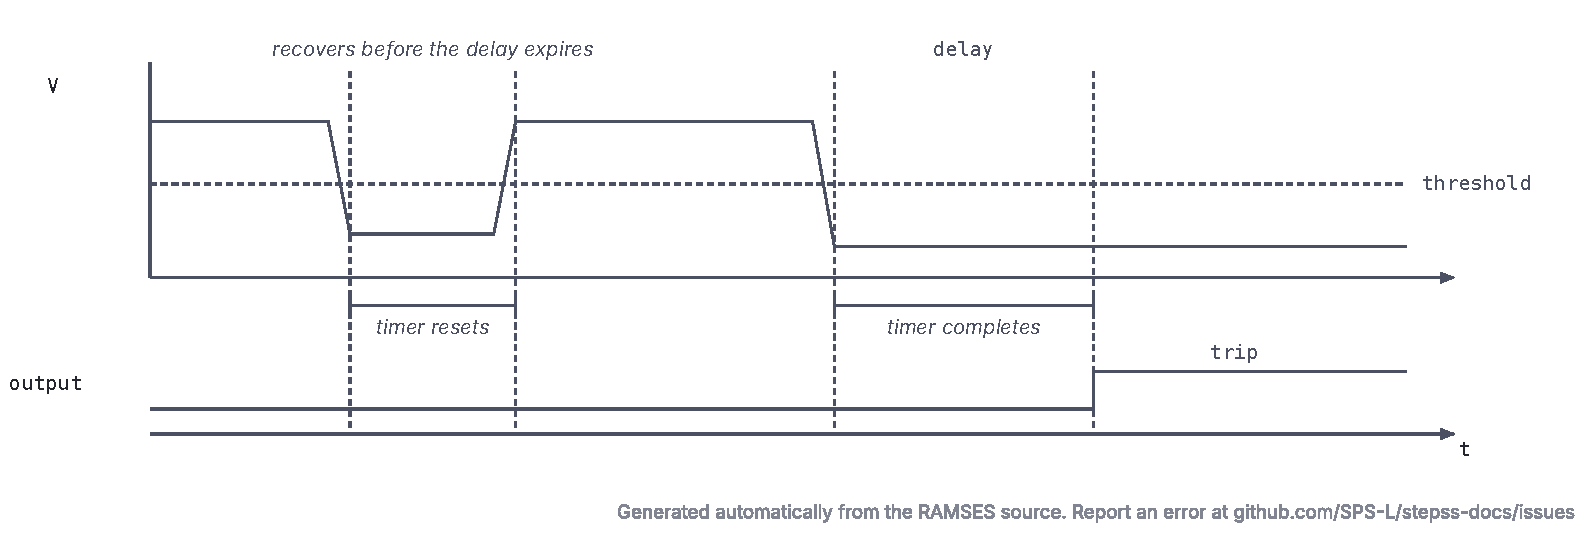
\includegraphics[width=0.98\linewidth]{figures/dctl-relay-timing-light}
\caption{Definite-time relay timing diagram.}
\end{figure}

\section{\texorpdfstring{UVPROT (\texttt{dctl\_uvprot}): Under-Voltage Protection Relay}{UVPROT (dctl\_uvprot): Under-Voltage Protection Relay}}\label{model-dctl-prot:uvprot-dctl_uvprot-under-voltage-protection-relay}

\subsection{Description}\label{model-dctl-prot:description}

Trips a \textbf{generator or injector} when the voltage at a monitored bus falls below a threshold for a sustained time delay. This models definite-time under-voltage protection relays.

\subsection{Logic Description}\label{model-dctl-prot:logic-description}

The relay monitors voltage \(V_{meas}\) at a specified bus:

\[\text{if } V_{meas} < V_{\min}: \quad \text{start timer}\]
\[\text{if timer} \ge T_{delay}: \quad \text{trip generator}, \quad \text{state} \leftarrow -1 \text{ (latched)}\]

Once tripped (\texttt{w(8)\ =\ -1}), the controller is permanently latched and takes no further action.

\subsection{Parameters}\label{model-dctl-prot:parameters}

\begin{small}\begin{longtable}[]{@{}lll@{}}
\toprule\noalign{}
Field & Working variable & Description \\
\midrule\noalign{}
\endhead
\bottomrule\noalign{}
\endlastfoot
\texttt{bus\_name} & \texttt{w(1)} & Monitored bus name \\
\texttt{gen\_name} & \texttt{w(2)} & Generator/injector to trip \\
\texttt{Vmin} & \texttt{w(3)} & Under-voltage pickup threshold (pu) \\
\texttt{T\_delay} & \texttt{w(4)} & Time delay before tripping (s) \\
\end{longtable}\end{small}

Internal variables: \texttt{w(5)} = measured voltage, \texttt{w(6)} = start time of violation, \texttt{w(7)} = simulation time, \texttt{w(8)} = controller state.

\subsection{Usage Example}\label{model-dctl-prot:usage-example}

\begin{Verbatim}
DCTL  UVPROT  UV_GEN1
      # bus: monitored bus
      BUS_HV
      # generator: must name an existing synchronous machine; RAMSES 3.84 does not use it to pick the tripped unit
      GEN1
      # Vmin: voltage threshold, 0 < Vmin <= 1 (pu)
      0.85
      # T_delay: time below Vmin before tripping, > 0 (s)
      0.5
;
\end{Verbatim}

\begin{center}\rule{0.5\linewidth}{0.5pt}\end{center}

\section{\texorpdfstring{UVLS (\texttt{dctl\_uvls}): Under-Voltage Load Shedding}{UVLS (dctl\_uvls): Under-Voltage Load Shedding}}\label{model-dctl-prot:uvls-dctl_uvls-under-voltage-load-shedding}

\subsection{Description}\label{model-dctl-prot:description-1}

Sheds load in \textbf{multiple steps} in response to sustained voltage depression. The controller integrates the area between the measured voltage and a threshold (energy integral criterion) and triggers load shedding when the area exceeds a limit \(C\). This prevents unnecessary shedding for short transient dips.

After each shedding step, the controller resets the integral and waits a minimum delay before the next step.

\subsection{Logic Description}\label{model-dctl-prot:logic-description-1}

Area integral (trapezoidal):

\[A(t) = \int_{t_{start}}^{t} \max(V_{th} - V_{meas}, 0) \, dt'\]

Shedding condition:

\[\text{if } A \ge C \text{ and } (t - t_{last}) \ge T_{\min}: \quad \text{shed load step}\]

Amount shed per step (bounded):

\[\Delta P_{shed} = \text{clip}\left(K \cdot A, \; P_{\min,step}, \; P_{\max,step}\right)\]

Controller terminates when total shedding reaches the fraction \texttt{frac\_load} of initial load or when \texttt{max\_steps} is exhausted.

\subsection{Parameters}\label{model-dctl-prot:parameters-1}

\begin{small}\begin{longtable}[]{@{}
  >{\raggedright\arraybackslash}p{(\linewidth - 6\tabcolsep) * \real{0.2466}}
  >{\raggedright\arraybackslash}p{(\linewidth - 6\tabcolsep) * \real{0.2227}}
  >{\raggedright\arraybackslash}p{(\linewidth - 6\tabcolsep) * \real{0.5307}}
@{}}
\toprule\noalign{}
\begin{minipage}[b]{\linewidth}\raggedright
Field
\end{minipage} & \begin{minipage}[b]{\linewidth}\raggedright
Working variable
\end{minipage} & \begin{minipage}[b]{\linewidth}\raggedright
Description
\end{minipage} \\
\midrule\noalign{}
\endhead
\bottomrule\noalign{}
\endlastfoot
\texttt{bus\_name} & \texttt{w(1)} & Monitored bus \\
\texttt{load\_name} & \texttt{w(2)} & Controlled load (injector) \\
\texttt{V\_th} & \texttt{w(3)} & Voltage threshold (pu) \\
\texttt{C} & \texttt{w(4)} & Maximum area \(\int(V_{th}-V) \, dt\) before shedding (pu\ensuremath{\cdot}s) \\
\texttt{T\_min} & \texttt{w(5)} & Minimum delay between steps (s) \\
\texttt{T\_max} & \texttt{w(6)} & Maximum delay between steps (s) \\
\texttt{frac\_load} & \texttt{w(7)} & Maximum fraction of load that may be shed \\
\texttt{K} & \texttt{w(8)} & Gain: area \ensuremath{\rightarrow} shed amount \\
\texttt{P\_min\_step} & \texttt{w(9)} & Minimum load shedding per step (MW) \\
\texttt{P\_max\_step} & \texttt{w(10)} & Maximum load shedding per step (MW) \\
\texttt{max\_steps} & \texttt{w(11)} & Maximum number of shedding steps \\
\end{longtable}\end{small}

Internal variables: \texttt{w(12)}--\texttt{w(18)} (previous voltage, timers, area accumulator, step counter, total shed).

\subsection{Usage Example}\label{model-dctl-prot:usage-example-1}

\begin{Verbatim}
DCTL  UVLS  UVLS1
      # bus: monitored bus
      BUS_MV
      # load: injector shed by the controller (needs parameters P0 and Q0)
      LOAD1
      # V_th: voltage threshold (pu)
      0.90
      # C: area of voltage deficit that triggers shedding (pu s)
      0.5
      # T_min: minimum delay from arming to shedding (s)
      5.0
      # T_max: maximum delay from arming; shedding is forced after it (s)
      20.0
      # frac_load: fraction of the load that may be shed, capped at 1
      0.3
      # K: gain: shed amount per unit of mean voltage deficit (MW/pu)
      2.0
      # P_min_step: minimum load shed per step (MW)
      5.0
      # P_max_step: maximum load shed per step (MW)
      50.0
      # max_steps: maximum number of shedding steps
      5
;
\end{Verbatim}

\begin{center}\rule{0.5\linewidth}{0.5pt}\end{center}

\section{\texorpdfstring{\texttt{FRT} (\texttt{dctl\_FRT}): Fault Ride-Through Controller}{FRT (dctl\_FRT): Fault Ride-Through Controller}}\label{model-dctl-prot:frt-dctl_frt-fault-ride-through-controller}

\subsection{Description}\label{model-dctl-prot:description-2}

Implements a \textbf{piecewise-linear voltage--time FRT envelope} for an inverter-based generator (IBG). It monitors the bus voltage of the controlled injector and trips the unit if the voltage stays below the FRT envelope longer than allowed by the characteristic.

The FRT envelope is defined by four (voltage, time) breakpoints: \((V_1, t_1), (V_2, t_2), (V_3, t_3), (V_4)\). If the voltage is above the envelope at all times, no action is taken. If it falls below the envelope for more than the corresponding time limit, the unit is tripped.

\subsection{Logic Description}\label{model-dctl-prot:logic-description-2}

The FRT curve defines the minimum voltage \(V(t)\) that must be sustained:

\begin{small}\begin{longtable}[]{@{}ll@{}}
\toprule\noalign{}
Segment & Condition \\
\midrule\noalign{}
\endhead
\bottomrule\noalign{}
\endlastfoot
\(V \ge V_1\) & Always ride-through \\
\(V_2 \le V < V_1\) & Must recover within \(t_1\) s \\
\(V_3 \le V < V_2\) & Must recover within \(t_2\) s \\
\(V_4 \le V < V_3\) & Must recover within \(t_3\) s \\
\(V < V_4\) & Immediate trip \\
\end{longtable}\end{small}

Two internal timers (\texttt{w(8)}, \texttt{w(9)}) track time spent in violation zones.

\subsection{Parameters}\label{model-dctl-prot:parameters-2}

\begin{small}\begin{longtable}[]{@{}
  >{\raggedright\arraybackslash}p{(\linewidth - 6\tabcolsep) * \real{0.2057}}
  >{\raggedright\arraybackslash}p{(\linewidth - 6\tabcolsep) * \real{0.2434}}
  >{\raggedright\arraybackslash}p{(\linewidth - 6\tabcolsep) * \real{0.5509}}
@{}}
\toprule\noalign{}
\begin{minipage}[b]{\linewidth}\raggedright
Field
\end{minipage} & \begin{minipage}[b]{\linewidth}\raggedright
Working variable
\end{minipage} & \begin{minipage}[b]{\linewidth}\raggedright
Description
\end{minipage} \\
\midrule\noalign{}
\endhead
\bottomrule\noalign{}
\endlastfoot
\texttt{inj\_name} & \texttt{w(10)} & Controlled injector \\
\texttt{Val1} & \texttt{w(1)} & Voltage threshold 1 (pu), upper FRT boundary \\
\texttt{t1} & \texttt{w(2)} & Time limit for zone 1 (s) \\
\texttt{Val2} & \texttt{w(3)} & Voltage threshold 2 (pu) \\
\texttt{t2} & \texttt{w(4)} & Time limit for zone 2 (s) \\
\texttt{Val3} & \texttt{w(5)} & Voltage threshold 3 (pu) \\
\texttt{t3} & \texttt{w(6)} & Time limit for zone 3 (s) \\
\texttt{Val4} & \texttt{w(7)} & Voltage threshold 4 (pu), below this: trip immediately \\
\end{longtable}\end{small}

8 fields required. Field 1 is the injector name, fields 2--8 map to \texttt{Val1,\ t1,\ Val2,\ t2,\ Val3,\ t3,\ Val4}.

\subsection{Usage Example}\label{model-dctl-prot:usage-example-2}

\begin{Verbatim}
DCTL  FRT  FRT_WTG1
      # injector: injector tripped by the relay
      WT1
      # Val1: trip voltage between t1 and t2 after timer 1 starts (pu)
      0.30
      # t1: end of the no-trip period of timer 1 (s)
      0.15
      # Val2: trip voltage after t2 on timer 1 (pu)
      0.70
      # t2: time on timer 1 from which Val2 applies (s)
      0.5
      # Val3: voltage below which timer 1 starts; must be below Val4 (pu)
      0.50
      # t3: time on timer 2 from which Val4 applies (s)
      1.5
      # Val4: voltage below which timer 2 starts; both timers reset when the voltage rises above it (pu)
      0.90
;
\end{Verbatim}

\begin{center}\rule{0.5\linewidth}{0.5pt}\end{center}

\section{dctl\_injprot: Injector Protection}\label{model-dctl-prot:dctl_injprot-injector-protection}

\begin{docsnote}{Note}

Callable since 3.79. Earlier releases compiled this model under no name, so a data file referring to it was rejected.

\end{docsnote}

\subsection{Description}\label{model-dctl-prot:description-3}

A \textbf{generic injector protection} relay that monitors any observable variable of an injector (e.g., current magnitude, active power, reactive power) and trips the injector if the variable goes outside prescribed bounds for a sustained time.

The controller identifies the variable to monitor by name from the injector's observable list, making it flexible and applicable to any injector model.

\subsection{Logic Description}\label{model-dctl-prot:logic-description-3}

\[\text{if } x_{obs} < L_{lower} \text{ or } x_{obs} > L_{upper}: \quad \text{start timer}\]
\[\text{if timer} \ge T_{trip}: \quad \text{trip injector}, \quad \text{state} \leftarrow -1\]

The controller latches once tripped and cannot reset. State variable \texttt{w(7)}:
- \texttt{1} = active (monitoring)
- \texttt{0} = idle (within bounds)
- \texttt{\ensuremath{-}1} = already tripped

\subsection{Parameters}\label{model-dctl-prot:parameters-3}

\begin{small}\begin{longtable}[]{@{}
  >{\raggedright\arraybackslash}p{(\linewidth - 6\tabcolsep) * \real{0.2589}}
  >{\raggedright\arraybackslash}p{(\linewidth - 6\tabcolsep) * \real{0.2219}}
  >{\raggedright\arraybackslash}p{(\linewidth - 6\tabcolsep) * \real{0.5192}}
@{}}
\toprule\noalign{}
\begin{minipage}[b]{\linewidth}\raggedright
Field
\end{minipage} & \begin{minipage}[b]{\linewidth}\raggedright
Working variable
\end{minipage} & \begin{minipage}[b]{\linewidth}\raggedright
Description
\end{minipage} \\
\midrule\noalign{}
\endhead
\bottomrule\noalign{}
\endlastfoot
\texttt{inj\_name} & \texttt{w(1)} & Monitored/controlled injector name \\
\texttt{var\_name} & \texttt{w(2)} & Observable variable name (from injector's observable list) \\
\texttt{lower\_bound} & \texttt{w(3)} & Lower bound for the variable \\
\texttt{upper\_bound} & \texttt{w(4)} & Upper bound for the variable \\
\texttt{T\_trip} & \texttt{w(5)} & Time out-of-bounds before tripping (s) \\
\end{longtable}\end{small}

5 fields required.

\subsection{Usage Example}\label{model-dctl-prot:usage-example-3}

\begin{Verbatim}
DCTL  injprot  PROT_WTG1
      # injector: injector tripped by the relay
      WT1
      # observable: name of an observable of that injector's model
      vt
      # lower_bound: lower bound on the observable, below upper_bound
      0.85
      # upper_bound: upper bound on the observable
      1.15
      # T_trip: read but not used in RAMSES 3.84, where the trip delay is fixed at 1 s (s)
      1.0
;
\end{Verbatim}

\begin{center}\rule{0.5\linewidth}{0.5pt}\end{center}

\section{dctl\_losprot: Loss-of-Synchronism Protection}\label{model-dctl-prot:dctl_losprot-loss-of-synchronism-protection}

\begin{docsnote}{Note}

Callable since 3.79. Earlier releases compiled this model under no name, so a data file referring to it was rejected.

\end{docsnote}

\subsection{Description}\label{model-dctl-prot:description-4}

Trips a \textbf{synchronous generator} when its rotor speed exceeds a maximum threshold for a sustained time, detecting loss of synchronism (pole slipping). The controller monitors the machine's per-unit rotor speed \(\omega\) and triggers disconnection when \(\omega > \omega_{max}\) for longer than the specified time delay.

\subsection{Logic Description}\label{model-dctl-prot:logic-description-4}

\[\text{if } \omega > \omega_{max}: \quad \text{start timer}\]
\[\text{if timer} \ge T_{delay}: \quad \text{trip generator}, \quad \text{state} \leftarrow -1\]

The timer resets if the speed returns within bounds. The controller latches permanently after tripping.

\subsection{Parameters}\label{model-dctl-prot:parameters-4}

\begin{small}\begin{longtable}[]{@{}lll@{}}
\toprule\noalign{}
Field & Working variable & Description \\
\midrule\noalign{}
\endhead
\bottomrule\noalign{}
\endlastfoot
\texttt{gen\_name} & \texttt{w(1)} & Controlled synchronous generator name \\
\texttt{omega\_max} & \texttt{w(2)} & Maximum rotor speed threshold (pu) \\
\texttt{T\_delay} & \texttt{w(3)} & Time delay before tripping (s) \\
\end{longtable}\end{small}

3 fields required. Internal variables: \texttt{w(4)} = measured speed, \texttt{w(5)} = violation start time, \texttt{w(6)} = current time, \texttt{w(7)} = state.

\subsection{Usage Example}\label{model-dctl-prot:usage-example-4}

\begin{Verbatim}
DCTL  LOSPROT  LOS_GEN2
      # generator: synchronous machine tripped by the relay
      GEN2
      # omega_max: speed threshold, > 0 (pu)
      1.05
      # T_delay: time above omega_max before tripping, >= 0 (s)
      0.2
;
\end{Verbatim}

\begin{center}\rule{0.5\linewidth}{0.5pt}\end{center}

\section{\texorpdfstring{line\_prot (\texttt{dctl\_line\_prot}): Line Overcurrent Protection}{line\_prot (dctl\_line\_prot): Line Overcurrent Protection}}\label{model-dctl-prot:line_prot-dctl_line_prot-line-overcurrent-protection}

The data-file model name is \texttt{line\_prot} (or \texttt{dctl\_line\_prot}). RAMSES adds the \texttt{dctl\_} prefix automatically.

\subsection{Description}\label{model-dctl-prot:description-5}

Monitors the \textbf{apparent power flow on a set of lines} and trips them if they exceed their thermal rating (with a configurable oversize factor). It is designed to protect multiple lines simultaneously and disconnects any line whose flow exceeds \texttt{oversize\_factor\ \ensuremath{\times}\ S\_max}.

The controller uses RAMSES' internal \texttt{smax\_bra} array (maximum apparent power ratings from the network data) and reads real-time power flows via \texttt{pqbra}.

\subsection{Logic Description}\label{model-dctl-prot:logic-description-5}

For each monitored branch \(k\):

\[\text{if } |S_k| > \text{oversize\_factor} \times S_{max,k}: \quad \text{disconnect branch } k\]

The action is immediate (no time delay); the oversize factor allows temporary overloads.

\subsection{Parameters}\label{model-dctl-prot:parameters-5}

\begin{small}\begin{longtable}[]{@{}
  >{\raggedright\arraybackslash}p{(\linewidth - 6\tabcolsep) * \real{0.2553}}
  >{\raggedright\arraybackslash}p{(\linewidth - 6\tabcolsep) * \real{0.2324}}
  >{\raggedright\arraybackslash}p{(\linewidth - 6\tabcolsep) * \real{0.5124}}
@{}}
\toprule\noalign{}
\begin{minipage}[b]{\linewidth}\raggedright
Field
\end{minipage} & \begin{minipage}[b]{\linewidth}\raggedright
Working variable
\end{minipage} & \begin{minipage}[b]{\linewidth}\raggedright
Description
\end{minipage} \\
\midrule\noalign{}
\endhead
\bottomrule\noalign{}
\endlastfoot
\texttt{oversize\_factor} & \texttt{w(1)} & Allowed overload factor (e.g., 1.05 = 5\% overload permitted) \\
\texttt{nb\_lines} & \texttt{w(2)} & Number of protected lines \\
\texttt{line\_1}, \ldots{} & \texttt{w(3-)} & Names of protected branches (space-separated) \\
\end{longtable}\end{small}

\subsection{Usage Example}\label{model-dctl-prot:usage-example-5}

\begin{Verbatim}
DCTL  line_prot  LINEPROT1
      # oversize: trip threshold as a multiple of the branch rating
      1.05
      # nb_lines: number of protected branches
      2
      # branch: protected branch
      L1-L2
      # branch: protected branch
      L3-L4
;
\end{Verbatim}

\begin{center}\rule{0.5\linewidth}{0.5pt}\end{center}

\section{\texorpdfstring{\texttt{PST} (\texttt{dctl\_pst}): Phase-Shifting Transformer Control}{PST (dctl\_pst): Phase-Shifting Transformer Control}}\label{model-dctl-prot:pst-dctl_pst-phase-shifting-transformer-control}

\subsection{Description}\label{model-dctl-prot:description-6}

Controls the phase angle (and thus the \textbf{active power flow}) of a phase-shifting transformer (PST) to regulate power flow on a monitored branch. It is structurally identical to \texttt{dctl\_ltc} but acts on the PST angle rather than on voltage: the deadband is in MW (or pu power), and the controller moves the tap to keep active power within a band around the setpoint.

\subsection{Logic Description}\label{model-dctl-prot:logic-description-6}

Let \(P_{meas}\) be the active power flow on the monitored branch and \(P_{set}\) the setpoint (initialised at \(t=0\)):

\[\text{if } |P_{meas} - P_{set}| > \delta P: \quad \text{start timer}\]
\[\text{if timer} \ge \tau_{delay}: \quad \text{advance/retard PST angle by } \Delta\phi\]

The direction parameter defines whether increasing the tap increases or decreases power flow.

\subsection{Parameters}\label{model-dctl-prot:parameters-6}

\begin{small}\begin{longtable}[]{@{}lll@{}}
\toprule\noalign{}
Field & Working variable & Description \\
\midrule\noalign{}
\endhead
\bottomrule\noalign{}
\endlastfoot
\texttt{pst\_branch} & \texttt{w(1)} & PST branch name (must be type \texttt{trfo}) \\
\texttt{mon\_branch} & \texttt{w(2)} & Monitored branch for power flow \\
\texttt{direction} & \texttt{w(3)} & Sign convention for power vs.~Angle \\
\texttt{ratio\_min} & \texttt{w(4)} & Minimum PST ratio (pu) \\
\texttt{ratio\_max} & \texttt{w(5)} & Maximum PST ratio (pu) \\
\texttt{nb\_positions} & \texttt{w(6)} & Number of positions \\
\texttt{half\_deadband} & \texttt{w(7)} & Power half-deadband (pu) \\
\texttt{delay\_first} & \texttt{w(8)} & First change delay (s) \\
\texttt{delay\_next} & \texttt{w(9)} & Subsequent change delay (s) \\
\end{longtable}\end{small}

9 fields required. Internal variables: \texttt{w(10)} = power setpoint, \texttt{w(11)} = time of last change, \texttt{w(12)} = active delay, \texttt{w(13)} = state.

\subsection{Usage Example}\label{model-dctl-prot:usage-example-6}

\begin{Verbatim}
DCTL  PST  PST_L1
      # branch: phase-shifting transformer, which is also the branch whose power is controlled
      PST-TR1
      # mon_branch: not read by RAMSES 3.84: any name
      LINE-MON
      # direction: sign of the phase change that raises the power (only the sign is used, 0 is refused)
      1
      # phase_min: minimum phase angle (deg)
      -30.
      # phase_max: maximum phase angle (deg)
      30.
      # nb_positions: number of tap positions, at least 2
      21
      # half_deadband: half of the power deadband (pu)
      0.02
      # delay_first: delay before the first tap change (s)
      30.0
      # delay_next: delay between subsequent tap changes (s)
      10.0
;
\end{Verbatim}

\begin{center}\rule{0.5\linewidth}{0.5pt}\end{center}

\section{\texorpdfstring{\texttt{RT} (\texttt{dctl\_rt}): Real-Time Simulation Control}{RT (dctl\_rt): Real-Time Simulation Control}}\label{model-dctl-prot:rt-dctl_rt-real-time-simulation-control}

\subsection{Description}\label{model-dctl-prot:description-7}

Forces the RAMSES simulation to track \textbf{wall-clock time} at a configurable ratio, enabling hardware-in-the-loop (HIL) or real-time simulation testing. A ratio of 1.0 means the simulation runs in exact real time; a ratio of 2.0 allows the simulation to run up to twice as fast as real time (useful for digital twin applications).

An optional over-run tolerance parameter \texttt{allowed\_overrun} specifies how far the simulation may lag behind real time before an error is triggered.

\subsection{Parameters}\label{model-dctl-prot:parameters-7}

\begin{small}\begin{longtable}[]{@{}
  >{\raggedright\arraybackslash}p{(\linewidth - 6\tabcolsep) * \real{0.2500}}
  >{\raggedright\arraybackslash}p{(\linewidth - 6\tabcolsep) * \real{0.2450}}
  >{\raggedright\arraybackslash}p{(\linewidth - 6\tabcolsep) * \real{0.5050}}
@{}}
\toprule\noalign{}
\begin{minipage}[b]{\linewidth}\raggedright
Field
\end{minipage} & \begin{minipage}[b]{\linewidth}\raggedright
Working variable
\end{minipage} & \begin{minipage}[b]{\linewidth}\raggedright
Description
\end{minipage} \\
\midrule\noalign{}
\endhead
\bottomrule\noalign{}
\endlastfoot
\texttt{ratio} & \texttt{w(1)} & Ratio to real time (1.0 = real time, \textgreater1 = faster) \\
\texttt{allowed\_overrun} & \texttt{w(2)} & Allowed over-run before error (s), optional \\
\end{longtable}\end{small}

1 or 2 fields. Only one \texttt{DCTL\ RT} controller may be active per simulation.

Observable: \texttt{elapsed} (wall-clock elapsed time in seconds).

\subsection{Usage Example}\label{model-dctl-prot:usage-example-7}

\begin{Verbatim}
DCTL  RT  RT_CTL
      # ratio: simulated time per second of wall time
      1.0
      # lead_time: how far the simulation may run ahead of scaled wall time (optional, default 0) (s)
      0.01
;
\end{Verbatim}

\begin{center}\rule{0.5\linewidth}{0.5pt}\end{center}

\section{\texorpdfstring{\texttt{dctl\_hvdc\_lim}: HVDC LCC Limiter/Controller}{dctl\_hvdc\_lim: HVDC LCC Limiter/Controller}}\label{model-dctl-prot:dctl_hvdc_lim-hvdc-lcc-limitercontroller}

\begin{docsnote}{Note}

Callable since 3.79. Earlier releases compiled this model under no name, so a data file referring to it was rejected.

\end{docsnote}

\subsection{Description}\label{model-dctl-prot:description-8}

A discrete controller that \textbf{supervises and adjusts an LCC-HVDC link} (\texttt{twop\_HVDC\_LCC}) by:
- Moving rectifier and inverter transformer tap changers to maintain firing and extinction angles within desired ranges
- Triggering reduced-current or blocked operation when AC voltages are too low for normal commutation
- Setting the \texttt{alphamin}, \texttt{gammamin}, and \texttt{Idred} parameters of the HVDC model

It interacts directly with the HVDC two-port model's internal parameters.

\subsection{Logic Description}\label{model-dctl-prot:logic-description-7}

\textbf{Rectifier tap changer}: if \(\alpha\) is outside \([\alpha_{min,des}, \alpha_{max,des}]\) for longer than \texttt{delay\_rect}, move rectifier transformer tap.

\textbf{Inverter tap changer}: if \(\gamma\) is outside \([\gamma_{min,des}, \gamma_{max,des}]\) for longer than \texttt{delay\_inv}, move inverter transformer tap.

\textbf{Reduced-current control}: when \(V_{dc}\) falls below \(V_{min,des}\) or \(V_{max,des}\) the controller switches the inverter to reduced-current mode (\texttt{inv\_ctl\ =\ -1}) and sets \(I_{red}\).

\textbf{Blocked operation}: if conditions are unrecoverable (very low AC voltage), the HVDC is blocked (\texttt{rec\_ctl\ =\ 3}, \texttt{inv\_ctl\ =\ 3}).

\subsection{Parameters}\label{model-dctl-prot:parameters-8}

\begin{small}\begin{longtable}[]{@{}
  >{\raggedright\arraybackslash}p{(\linewidth - 6\tabcolsep) * \real{0.2683}}
  >{\raggedright\arraybackslash}p{(\linewidth - 6\tabcolsep) * \real{0.2076}}
  >{\raggedright\arraybackslash}p{(\linewidth - 6\tabcolsep) * \real{0.5241}}
@{}}
\toprule\noalign{}
\begin{minipage}[b]{\linewidth}\raggedright
Field
\end{minipage} & \begin{minipage}[b]{\linewidth}\raggedright
Working variable
\end{minipage} & \begin{minipage}[b]{\linewidth}\raggedright
Description
\end{minipage} \\
\midrule\noalign{}
\endhead
\bottomrule\noalign{}
\endlastfoot
\texttt{hvdc\_name} & \texttt{w(1)} & Target HVDC two-port device name \\
\texttt{nr\_min} & \texttt{w(2)} & Minimum rectifier transformer ratio \\
\texttt{nr\_max} & \texttt{w(3)} & Maximum rectifier transformer ratio \\
\texttt{nr\_step} & \texttt{w(4)} & Rectifier tap step size \\
\texttt{ni\_min} & \texttt{w(5)} & Minimum inverter transformer ratio \\
\texttt{ni\_max} & \texttt{w(6)} & Maximum inverter transformer ratio \\
\texttt{ni\_step} & \texttt{w(7)} & Inverter tap step size \\
\texttt{alpha\_min\_des} & \texttt{w(8)} & Desired minimum firing angle (degrees) \\
\texttt{alpha\_max\_des} & \texttt{w(9)} & Desired maximum firing angle (degrees) \\
\texttt{gamma\_min\_des} & \texttt{w(10)} & Desired minimum extinction angle (degrees) \\
\texttt{gamma\_max\_des} & \texttt{w(11)} & Desired maximum extinction angle (degrees) \\
\texttt{V\_min\_des} & \texttt{w(12)} & Minimum desired DC voltage (kV) \\
\texttt{V\_max\_des} & \texttt{w(13)} & Maximum desired DC voltage (kV) \\
\texttt{delay\_rect} & \texttt{w(14)} & Delay between rectifier tap changes (s) \\
\texttt{delay\_inv} & \texttt{w(15)} & Delay between inverter tap changes (s) \\
\texttt{alphamin} & \texttt{w(16)} & Minimum firing angle limit (degrees) \\
\texttt{Idred} & \texttt{w(17)} & Reduced DC current (kA) \\
\texttt{gammamin} & \texttt{w(18)} & Minimum extinction angle (degrees) \\
\end{longtable}\end{small}

18 fields required. Internal variables: \texttt{w(19)}--\texttt{w(22)} (operation modes and tap-change timers).

\subsection{Usage Example}\label{model-dctl-prot:usage-example-8}

\begin{Verbatim}
DCTL  HVDC_LIM  HVDCLIM1
      # twop: HVDC_LCC two-port controlled
      HVDClink
      # nr_min: minimum rectifier transformer ratio
      0.85
      # nr_max: maximum rectifier transformer ratio
      1.15
      # nr_step: rectifier ratio step
      0.00625
      # ni_min: minimum inverter transformer ratio
      0.85
      # ni_max: maximum inverter transformer ratio
      1.15
      # ni_step: inverter ratio step
      0.00625
      # alpha_min_des: lower edge of the desired firing angle band (deg)
      15.0
      # alpha_max_des: upper edge of the desired firing angle band (deg)
      18.0
      # gamma_min_des: lower edge of the desired extinction angle band (deg)
      15.0
      # gamma_max_des: upper edge of the desired extinction angle band (deg)
      18.0
      # V_min_des: lower edge of the desired DC voltage band (kV)
      400.0
      # V_max_des: upper edge of the desired DC voltage band (kV)
      600.0
      # delay_rect: delay between rectifier tap changes (s)
      10.0
      # delay_inv: delay between inverter tap changes (s)
      10.0
      # alphamin: minimum firing angle (deg)
      5.0
      # deltaI: DC current reduction when alpha reaches alphamin and the inverter takes current control (kA)
      0.0
      # gammamin: minimum extinction angle (deg)
      15.0
;
\end{Verbatim}
